\documentclass[12pt]{article}
% custom geometry
\usepackage[margin=1in]{geometry}

% customized titles for sections and subsections

% \usepackage[nodisplayskipstretch]{setspace}
\usepackage{setspace}
\onehalfspacing
%%% packages and libraries %%%
\usepackage{amsmath, amsthm, amssymb, amsfonts}
\usepackage{mathtools}
\usepackage{enumerate, enumitem}
\usepackage{algorithm, algpseudocode}
\usepackage{xparse}

%%% custom stats commands %%%
\newcommand{\simiid}{\overset{\scriptscriptstyle{\textrm{i.i.d.}}}{\sim}}
\newcommand{\indep}{\mathrel{\perp\!\!\!\perp}}
\newcommand{\estm}[2][]{\widehat{#2}_{#1}} % estimator
\newcommand{\iter}[2]{{#1}^{(#2)}} % iteration of algorithm

%%% custom math commands %%%
\newcommand{\tpose}[1]{#1^{\scriptstyle{\mathsf{T}}}} % transpose
\newcommand{\ctpose}[1]{#1^{\scriptstyle{\mathsf{H}}}} % conjugate transpose
\newcommand{\floor}[1]{\lfloor{#1}\rfloor}
\newcommand{\ceil}[1]{\lceil{#1}\rceil}

\DeclareMathOperator*{\argmax}{arg\,max}
\DeclareMathOperator*{\argmin}{arg\,min}
\DeclareMathOperator{\sign}{sign}
\DeclareMathOperator{\sgn}{sgn}
\DeclareMathOperator{\rank}{rank}
\DeclareMathOperator{\spn}{span}
\DeclareMathOperator{\tr}{tr}
\DeclareMathOperator{\supp}{supp}

% probability of event (optional subscript, blank by default)
\NewDocumentCommand{\prob}{ s O{} m }{
    \IfBooleanTF{#1}
        {\bbP_{#2}(#3)}              % \prob*{} (no resizing)
        {\bbP_{#2}\!\left(#3\right)} % \prob (auto-sizing)
}

% expectation (optional subscript, blank by default)
\NewDocumentCommand{\expec}{ s O{} m }{
    \IfBooleanTF{#1}
        {\bbE_{#2}[#3]}              % \expec*{} (no resizing)
        {\bbE_{#2}\!\left[#3\right]} % \expec (auto-sizing)
}

% variance (optional subscript, blank by default)
\NewDocumentCommand{\var}{ s O{} m }{
    \IfBooleanTF{#1}
        {\operatorname{Var}_{#2}[#3]}              % \var*{} (no resizing)
        {\operatorname{Var}_{#2}\!\left[#3\right]} % \var (auto-sizing)
}

% covariance (optional subscript, blank by default)
\NewDocumentCommand{\covar}{ s O{} m m }{
    \IfBooleanTF{#1}
        {\operatorname{Cov}_{#2}(#3, #4)}              % \covar*{} (no resizing)
        {\operatorname{Cov}_{#2}\!\left(#3, #4\right)} % \covar (auto-sizing)
}

% correlation (optional subscript, blank by default)
\NewDocumentCommand{\corr}{ s O{} m m }{
    \IfBooleanTF{#1}
        {\operatorname{corr}_{#2}(#3, #4)}              % \corr*{} (no resizing)
        {\operatorname{corr}_{#2}\!\left(#3, #4\right)} % \corr (auto-sizing)
}

% bias (optional subscript, blank by default)
\NewDocumentCommand{\bias}{ s O{} m }{
    \IfBooleanTF{#1}
        {\operatorname{bias}_{#2}(#3)}              % \bias*{} (no resizing)
        {\operatorname{bias}_{#2}\!\left(#3\right)} % \bias (auto-sizing)
}

% MSE (optional subscript, blank by default)
\NewDocumentCommand{\MSE}{ s O{} m }{
    \IfBooleanTF{#1}
        {\operatorname{MSE}_{#2}(#3)}              % \MSE*{} (no resizing)
        {\operatorname{MSE}_{#2}\!\left(#3\right)} % \MSE (auto-sizing)
}

% "full" derivative 
\NewDocumentCommand{\dx}{ o }{
    \mathrm{d}
    \IfValueT{#1}{
        \IfBlankF{#1}{#1}
    }
}

% "full" derivative (fractional)
\NewDocumentCommand{\ddx}{ O{} m m }{
    \IfValueTF{#1}
        {\frac{\dx^{#1}#2}{\dx{#3^{#1}}}}
        {\frac{\dx{#2}}{\dx{#3}}}
}

% partial derivative
\NewDocumentCommand{\px}{ o }{
    \partial
    \IfValueT{#1}{
        \IfBlankF{#1}{#1}
    }
}

% partial derivative (fractional)
\NewDocumentCommand{\pdx}{ O{} m m }{
    \IfValueTF{#1}
        {\frac{\px^{#1}#2}{\px{#3^{#1}}}}
        {\frac{\px{#2}}{\px{#3}}}
}

% inner product (optional base, blank by default)
\NewDocumentCommand{\innerprod}{ s O{} m m }{
    \IfBooleanTF{#1}
        {\langle{#3},{#4}\rangle_{#2}}            % \innerprod*{} (no resizing)       
        {\left\langle{#3},{#4}\right\rangle_{#2}} % \innerprod{}  (auto-sizing)
}

% norm (optional base, blank by default)
\NewDocumentCommand{\norm}{ s O{} m }{
    \IfBooleanTF{#1}
        {\lVert{#3}\rVert_{#2}}            % \norm*{} (no resizing)
        {\left\lVert{#3}\right\rVert_{#2}} % \norm{}  (auto-sizing)
}

% absolute value
\NewDocumentCommand{\abs}{ s m }{
    \IfBooleanTF{#1}
        {\lvert{#2}\rvert}            % \abs*{} (no resizing)
        {\left\lvert{#2}\right\rvert} % \abs{}  (auto-sizing)
}
%%% packages and libraries %%%
\usepackage{amsmath, amsthm, amssymb, amsfonts}
\usepackage{bm}

%%% mathbb alphabet %%%
\newcommand{\bbA}{\mathbb{A}}
\newcommand{\bbB}{\mathbb{B}}
\newcommand{\bbC}{\mathbb{C}}
\newcommand{\bbD}{\mathbb{D}}
\newcommand{\bbE}{\mathbb{E}}
\newcommand{\bbF}{\mathbb{F}}
\newcommand{\bbG}{\mathbb{G}}
\newcommand{\bbH}{\mathbb{H}}
\newcommand{\bbI}{\mathbb{I}}
\newcommand{\bbJ}{\mathbb{J}}
\newcommand{\bbK}{\mathbb{K}}
\newcommand{\bbL}{\mathbb{L}}
\newcommand{\bbM}{\mathbb{M}}
\newcommand{\bbN}{\mathbb{N}}
\newcommand{\bbO}{\mathbb{O}}
\newcommand{\bbP}{\mathbb{P}}
\newcommand{\bbQ}{\mathbb{Q}}
\newcommand{\bbR}{\mathbb{R}}
\newcommand{\bbS}{\mathbb{S}}
\newcommand{\bbT}{\mathbb{T}}
\newcommand{\bbU}{\mathbb{U}}
\newcommand{\bbV}{\mathbb{V}}
\newcommand{\bbW}{\mathbb{W}}
\newcommand{\bbX}{\mathbb{X}}
\newcommand{\bbY}{\mathbb{Y}}
\newcommand{\bbZ}{\mathbb{Z}}

%%% mathcal alphabet %%%
\newcommand{\calA}{\mathcal{A}}
\newcommand{\calB}{\mathcal{B}}
\newcommand{\calC}{\mathcal{C}}
\newcommand{\calD}{\mathcal{D}}
\newcommand{\calE}{\mathcal{E}}
\newcommand{\calF}{\mathcal{F}}
\newcommand{\calG}{\mathcal{G}}
\newcommand{\calH}{\mathcal{H}}
\newcommand{\calI}{\mathcal{I}}
\newcommand{\calJ}{\mathcal{J}}
\newcommand{\calK}{\mathcal{K}}
\newcommand{\calL}{\mathcal{L}}
\newcommand{\calM}{\mathcal{M}}
\newcommand{\calN}{\mathcal{N}}
\newcommand{\calO}{\mathcal{O}}
\newcommand{\calP}{\mathcal{P}}
\newcommand{\calQ}{\mathcal{Q}}
\newcommand{\calR}{\mathcal{R}}
\newcommand{\calS}{\mathcal{S}}
\newcommand{\calT}{\mathcal{T}}
\newcommand{\calU}{\mathcal{U}}
\newcommand{\calV}{\mathcal{V}}
\newcommand{\calW}{\mathcal{W}}
\newcommand{\calX}{\mathcal{X}}
\newcommand{\calY}{\mathcal{Y}}
\newcommand{\calZ}{\mathcal{Z}}

%%% mathsf alphabet (uppercase) %%%
\newcommand{\sfA}{\mathsf{A}}
\newcommand{\sfB}{\mathsf{B}}
\newcommand{\sfC}{\mathsf{C}}
\newcommand{\sfD}{\mathsf{D}}
\newcommand{\sfE}{\mathsf{E}}
\newcommand{\sfF}{\mathsf{F}}
\newcommand{\sfG}{\mathsf{G}}
\newcommand{\sfH}{\mathsf{H}}
\newcommand{\sfI}{\mathsf{I}}
\newcommand{\sfJ}{\mathsf{J}}
\newcommand{\sfK}{\mathsf{K}}
\newcommand{\sfL}{\mathsf{L}}
\newcommand{\sfM}{\mathsf{M}}
\newcommand{\sfN}{\mathsf{N}}
\newcommand{\sfO}{\mathsf{O}}
\newcommand{\sfP}{\mathsf{P}}
\newcommand{\sfQ}{\mathsf{Q}}
\newcommand{\sfR}{\mathsf{R}}
\newcommand{\sfS}{\mathsf{S}}
\newcommand{\sfT}{\mathsf{T}}
\newcommand{\sfU}{\mathsf{U}}
\newcommand{\sfV}{\mathsf{V}}
\newcommand{\sfW}{\mathsf{W}}
\newcommand{\sfX}{\mathsf{X}}
\newcommand{\sfY}{\mathsf{Y}}
\newcommand{\sfZ}{\mathsf{Z}}

%%% boldface math alphabet (uppercase) %%%
\newcommand{\bfA}{\mathbf{A}}
\newcommand{\bfB}{\mathbf{B}}
\newcommand{\bfC}{\mathbf{C}}
\newcommand{\bfD}{\mathbf{D}}
\newcommand{\bfE}{\mathbf{E}}
\newcommand{\bfF}{\mathbf{F}}
\newcommand{\bfG}{\mathbf{G}}
\newcommand{\bfH}{\mathbf{H}}
\newcommand{\bfI}{\mathbf{I}}
\newcommand{\bfJ}{\mathbf{J}}
\newcommand{\bfK}{\mathbf{K}}
\newcommand{\bfL}{\mathbf{L}}
\newcommand{\bfM}{\mathbf{M}}
\newcommand{\bfN}{\mathbf{N}}
\newcommand{\bfO}{\mathbf{O}}
\newcommand{\bfP}{\mathbf{P}}
\newcommand{\bfQ}{\mathbf{Q}}
\newcommand{\bfR}{\mathbf{R}}
\newcommand{\bfS}{\mathbf{S}}
\newcommand{\bfT}{\mathbf{T}}
\newcommand{\bfU}{\mathbf{U}}
\newcommand{\bfV}{\mathbf{V}}
\newcommand{\bfW}{\mathbf{W}}
\newcommand{\bfX}{\mathbf{X}}
\newcommand{\bfY}{\mathbf{Y}}
\newcommand{\bfZ}{\mathbf{Z}}

%%% boldface math alphabet (lowercase) %%%
\newcommand{\bfa}{\mathbf{a}}
\newcommand{\bfb}{\mathbf{b}}
\newcommand{\bfc}{\mathbf{c}}
\newcommand{\bfd}{\mathbf{d}}
\newcommand{\bfe}{\mathbf{e}}
\newcommand{\bff}{\mathbf{f}}
\newcommand{\bfg}{\mathbf{g}}
\newcommand{\bfh}{\mathbf{h}}
\newcommand{\bfi}{\mathbf{i}}
\newcommand{\bfj}{\mathbf{j}}
\newcommand{\bfk}{\mathbf{k}}
\newcommand{\bfl}{\mathbf{l}}
\newcommand{\bfm}{\mathbf{m}}
\newcommand{\bfn}{\mathbf{n}}
\newcommand{\bfo}{\mathbf{o}}
\newcommand{\bfp}{\mathbf{p}}
\newcommand{\bfq}{\mathbf{q}}
\newcommand{\bfr}{\mathbf{r}}
\newcommand{\bfs}{\mathbf{s}}
\newcommand{\bft}{\mathbf{t}}
\newcommand{\bfu}{\mathbf{u}}
\newcommand{\bfv}{\mathbf{v}}
\newcommand{\bfw}{\mathbf{w}}
\newcommand{\bfx}{\mathbf{x}}
\newcommand{\bfy}{\mathbf{y}}
\newcommand{\bfz}{\mathbf{z}}

%%% mathrm alphabet (uppercase) %%%
\newcommand{\rmA}{\mathrm{A}}
\newcommand{\rmB}{\mathrm{B}}
\newcommand{\rmC}{\mathrm{C}}
\newcommand{\rmD}{\mathrm{D}}
\newcommand{\rmE}{\mathrm{E}}
\newcommand{\rmF}{\mathrm{F}}
\newcommand{\rmG}{\mathrm{G}}
\newcommand{\rmH}{\mathrm{H}}
\newcommand{\rmI}{\mathrm{I}}
\newcommand{\rmJ}{\mathrm{J}}
\newcommand{\rmK}{\mathrm{K}}
\newcommand{\rmL}{\mathrm{L}}
\newcommand{\rmM}{\mathrm{M}}
\newcommand{\rmN}{\mathrm{N}}
\newcommand{\rmO}{\mathrm{O}}
\newcommand{\rmP}{\mathrm{P}}
\newcommand{\rmQ}{\mathrm{Q}}
\newcommand{\rmR}{\mathrm{R}}
\newcommand{\rmS}{\mathrm{S}}
\newcommand{\rmT}{\mathrm{T}}
\newcommand{\rmU}{\mathrm{U}}
\newcommand{\rmV}{\mathrm{V}}
\newcommand{\rmW}{\mathrm{W}}
\newcommand{\rmX}{\mathrm{X}}
\newcommand{\rmY}{\mathrm{Y}}
\newcommand{\rmZ}{\mathrm{Z}}

%%% mathrm alphabet (lowercase) %%%
\newcommand{\rma}{\mathrm{a}}
\newcommand{\rmb}{\mathrm{b}}
\newcommand{\rmc}{\mathrm{c}}
\newcommand{\rmd}{\mathrm{d}}
\newcommand{\rme}{\mathrm{e}}
\newcommand{\rmf}{\mathrm{f}}
\newcommand{\rmg}{\mathrm{g}}
\newcommand{\rmh}{\mathrm{h}}
\newcommand{\rmi}{\mathrm{i}}
\newcommand{\rmj}{\mathrm{j}}
\newcommand{\rmk}{\mathrm{k}}
\newcommand{\rml}{\mathrm{l}}
\newcommand{\rmm}{\mathrm{m}}
\newcommand{\rmn}{\mathrm{n}}
\newcommand{\rmo}{\mathrm{o}}
\newcommand{\rmp}{\mathrm{p}}
\newcommand{\rmq}{\mathrm{q}}
\newcommand{\rmr}{\mathrm{r}}
\newcommand{\rms}{\mathrm{s}}
\newcommand{\rmt}{\mathrm{t}}
\newcommand{\rmu}{\mathrm{u}}
\newcommand{\rmv}{\mathrm{v}}
\newcommand{\rmw}{\mathrm{w}}
\newcommand{\rmx}{\mathrm{x}}
\newcommand{\rmy}{\mathrm{y}}
\newcommand{\rmz}{\mathrm{z}}

%%% miscellaneous useful symbol commands %%%
\newcommand{\zeros}{\bm{0}}
\newcommand{\ones}{\bm{1}}
\newcommand{\bbeta}{\bm{\beta}}
\newcommand{\bepsilon}{\bm{\epsilon}}
\newcommand{\bmu}{\bm{\mu}}
\newcommand{\btheta}{\bm{\theta}}
\newcommand{\bSigma}{\bm{\Sigma}}

\newcommand{\T}{\scriptstyle{\sfT}}

\usepackage{caption,subcaption}
\usepackage{pifont}
\usepackage[numbers, square]{natbib}
\bibliographystyle{plainnat}

\usepackage{hyperref}
\usepackage{cleveref}
\usepackage{url}
\usepackage[dvipsnames]{xcolor}

\hypersetup{
    colorlinks = true,
    citecolor = ProcessBlue
    % linkcolor = RedOrange,
    % citecolor = BlueViolet,
    % urlcolor = ProcessBlue
}


% numbering for things by section
\renewcommand{\theequation}{\arabic{section}.\arabic{equation}}
\renewcommand{\thefigure}{\arabic{section}.\arabic{figure}}
\renewcommand{\thetable}{\arabic{section}.\arabic{table}}
\numberwithin{equation}{section}
\numberwithin{figure}{section}
\numberwithin{table}{section}

\newcommand{\FMNIST}{\texttt{Fashion-MNIST}\;}
\newcommand{\GP}{\mathcal{GP}}


\begin{document}

\begin{center}
    {\LARGE{\textbf{Gaussian Process Latent Variable Models for Simplifying Image Data}}}
    \vspace*{2cm}

    {\Large{Joey Hotz}}\\
    \vspace*{1cm}
    {\large{University of Toronto, Department of Statistical Sciences}}\\
    \vspace*{1cm}
    {\large{April 03, 2026}}

    \vfill

    \textbf{Team Information:} All aspects of this project (coding, writing the report, creating slides, project motivation, etc.) were done by Joey Hotz.\\
    \vspace*{0.5cm}
    All code is available on GitHub: \url{https://github.com/hotz1/STA2201-Final-Project}
\end{center}
\thispagestyle{empty}
\clearpage

\pagenumbering{arabic}
\setcounter{page}{1}

\section{Introduction}\label{sec:intro}

The overarching goal of this project is to investigate the properties of Gaussian Process Latent Variable Models (GP-LVMs), with a focus on the application of these models to dimension reduction in a high-dimensional data setting.

My personal motivation for choosing this topic for my report is that the GP-LVM method is an 

% My motivation for choosing this topic is 

\section{Methodology}\label{sec:methods}

In order to develop a full mathematical understanding of the GP-LVM methodology and how this method can be used for dimensionality reduction, we must first discuss two pre-requisite ideas which are crucial in motivating the GP-LVM. 

% In order to mathematically describe the GP-LVM methodology and how it relates to dimensionality reduction, we must first discuss the mathematics behind Gaussian Processes, as these are the key statistical objects used in creating these models.

\subsection{Probabilistic PCA}

\subsection{Gaussian Processes}

A Gaussian Process $\{X_{t}\}_{t \in T}$ is a stochastic process of random variables $\{X_{t}\}$ for $t$ in some pre-determined indexing set $T$ which has the property that the joint distribution of any any \emph{finite} collection of random variables from this process will be a multivariate Gaussian distribution. \cite{Rasmussen-GPML-2006} 

In more formal mathematical notation, for any collection of distinct indices $\{t_{1}, \dots, t_{N}\} \subset T$, the $N$-dimensional random vector $\begin{pmatrix}X_{t_{1}} & \cdots & X_{t_{N}}\end{pmatrix}^{\scriptstyle{\sfT}} \in \bbR^{N}$ follows a multivariate Gaussian distribution on $\bbR^{N}$. Note that by this definition, every individual random variable $X_{t}$ must follow a univariate Gaussian distribution. 

Gaussian Processes are commonly used in regression settings as a `surrogate model' for modelling unknown functions, as the framework for a Gaussian Process allows for a lot of flexibility wen learning an unknown function.



From a statistical perspective, a Gaussian Process defined on the indexing set $T$ is entirely specified by two functions; a \emph{mean function} $\mu: T \to \bbR$ which represents the expectation of the random variables, and a \emph{covariance kernel function} $k: T \times T \to \bbR$, which represents the covariance between the random variables \cite{Rasmussen-GPML-2006}. In most Gaussian Process regression settings, 



\subsection{Gaussian Process Latent Variable Models}

Now that we have covered the fundamentals of PPCA and Gaussian Processes, we may turn our attention towards the primary methodological focus of this report. 



\section{Data Description}\label{sec:data}

The primary image dataset which we use for our simulations involving this method is the \FMNIST dataset \cite{Fashion-MNIST}, which is a publicly-available benchmarking dataset used in a variety of machine learning tasks. The data is 

The primary dataset of interest for our simulation study is the \FMNIST dataset \cite{Fashion-MNIST}, which is a popular dataset for machine learning benchmarking. The choice of this dataset is primarily motivated by the simulations in \cite{GPLVM-2005}, which uses the `original' MNIST dataset containing handwritten digits.

The Fashion-MNIST dataset is built into many common machine learning software libraries by default, including \texttt{PyTorch} \cite{pytorch-library}.

\begin{figure}[!h]
\centering
    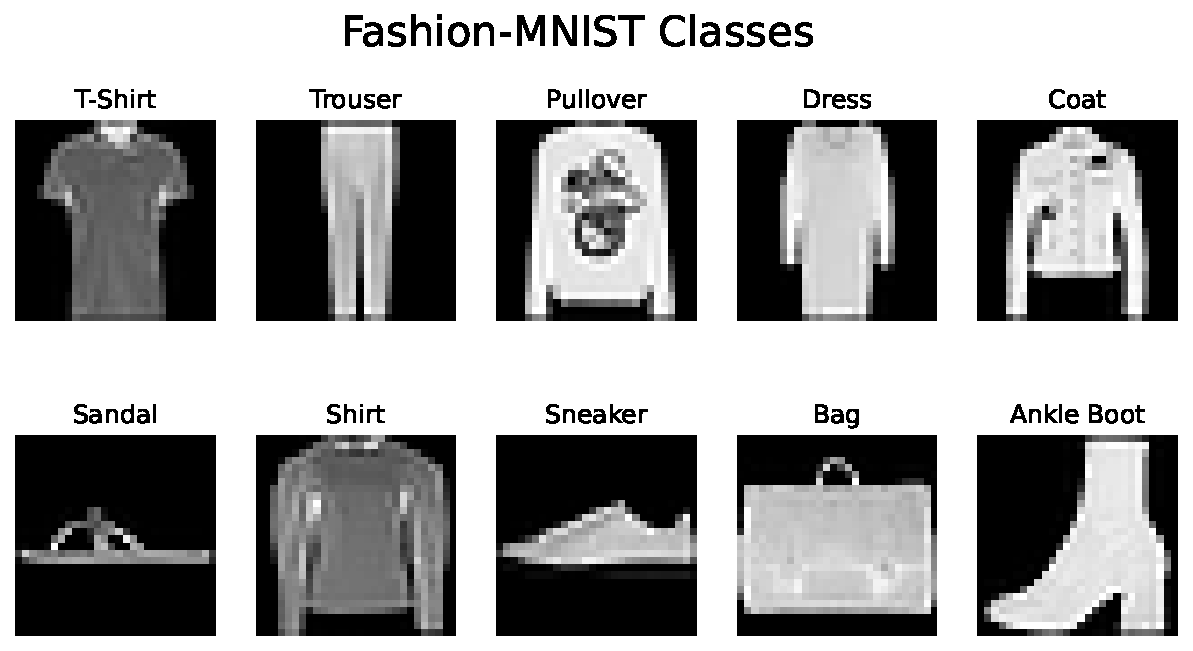
\includegraphics[width=0.95\linewidth]{../Code/outputs/fashion-mnist-examples.pdf}
    \caption{One example from each of the ten classes of clothing items in the \FMNIST dataset}
    \label{fig:fashion-MNIST-examples}
\end{figure}

\begin{figure}[!h]
\centering
    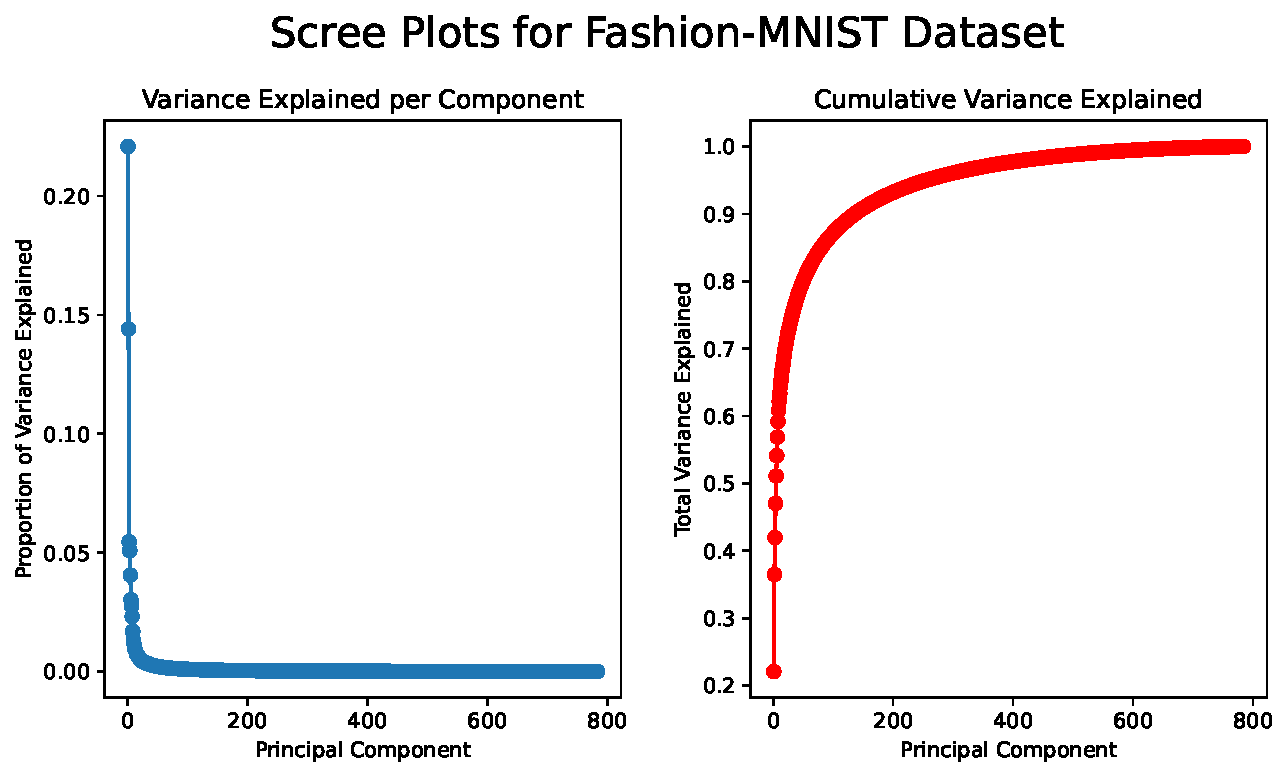
\includegraphics[width=0.95\linewidth]{../Code/outputs/fashion-mnist-scree.pdf}
    \caption{Scree plots for the principal components of the training data in the \FMNIST dataset}
    \label{fig:fashion-MNIST-scree}
\end{figure}

\begin{figure}[!h]
\centering
    \begin{subfigure}{0.48\textwidth}
        \centering
        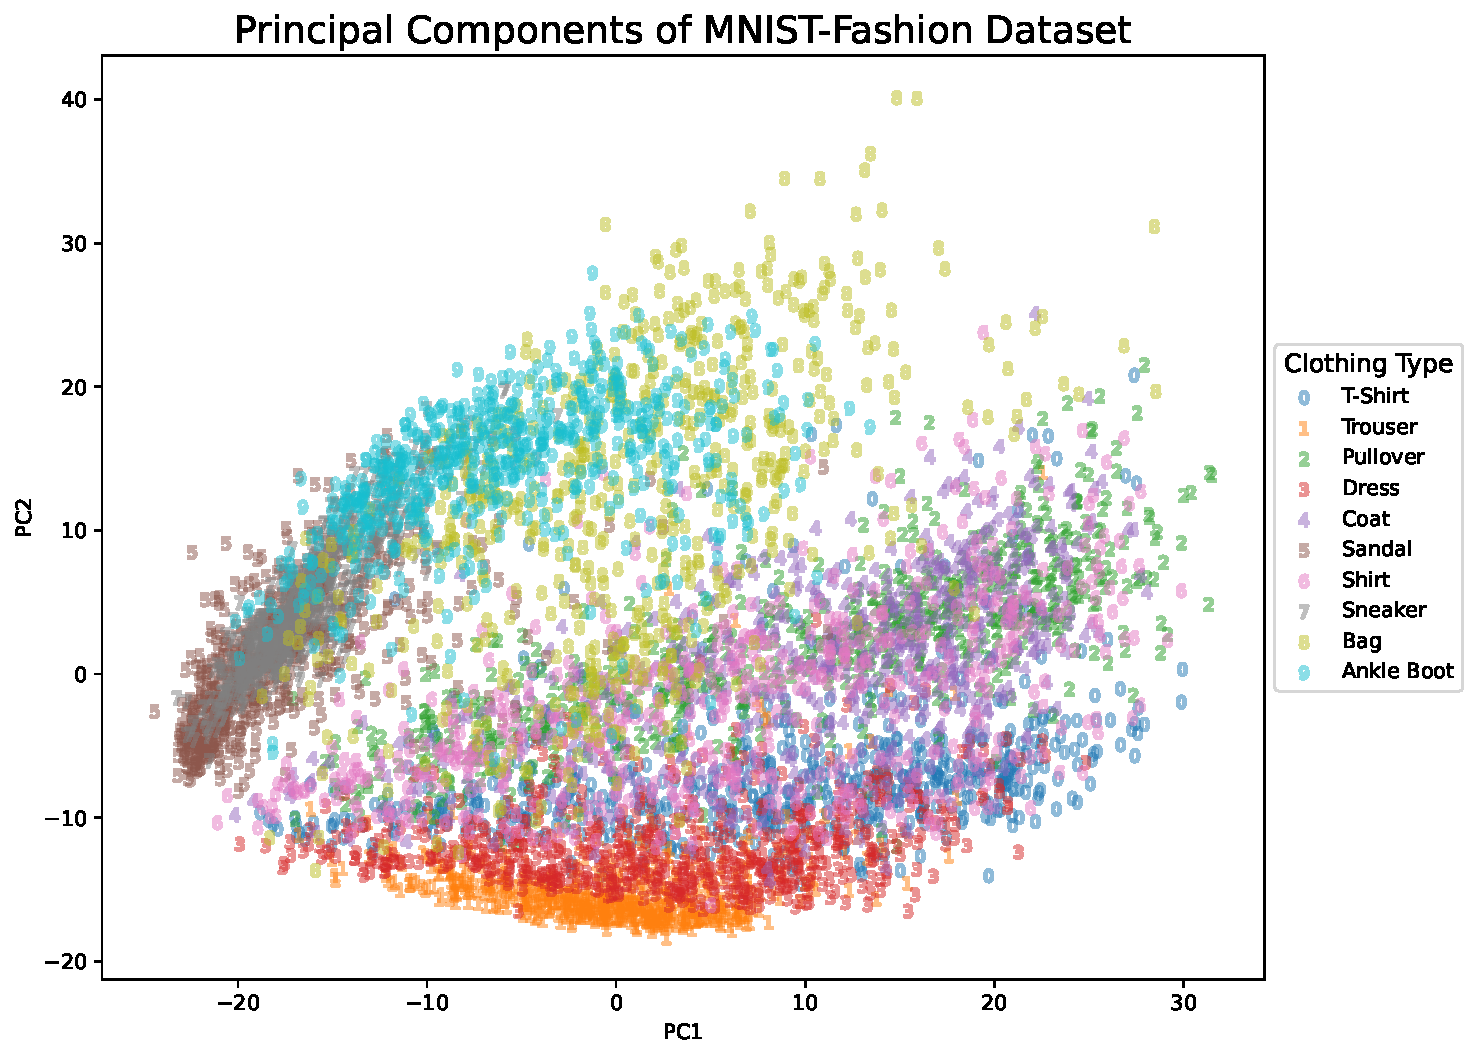
\includegraphics[width=\linewidth]{../Code/outputs/fashion-pca-2d.pdf}
        \caption{Top two principal components of clothing items in the \FMNIST dataset}
        \label{fig:fashion-pca-2d}
    \end{subfigure}
    \hfill
    \begin{subfigure}{0.48\textwidth}
        \centering
        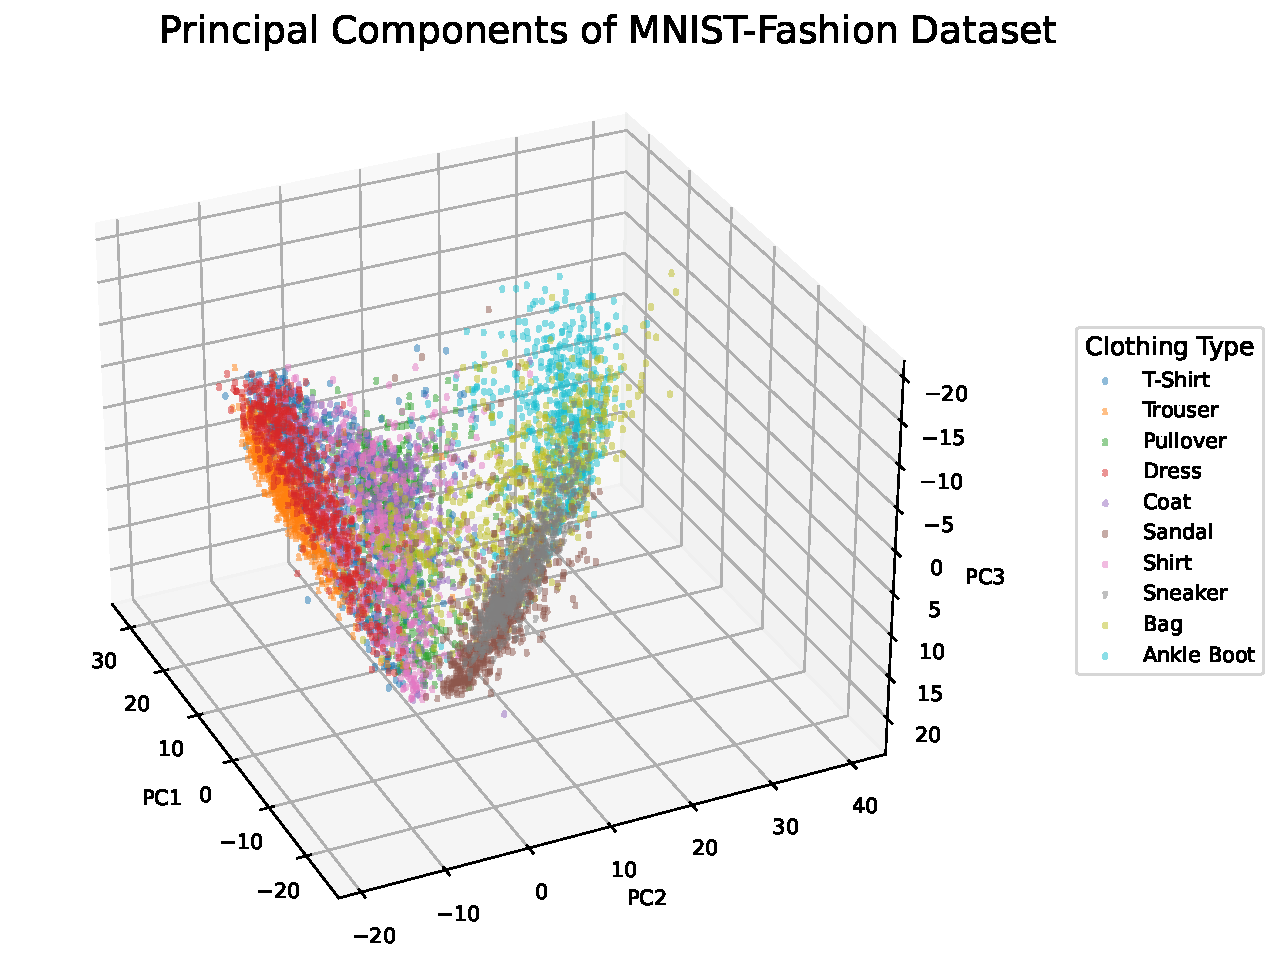
\includegraphics[width=\linewidth]{../Code/outputs/fashion-pca-3d.pdf}
        \caption{Top three principal components of clothing items in the \FMNIST dataset}
        \label{fig:fashion-pca-3d}
    \end{subfigure}
    \caption{Top principal components of clothing items, coloured by clothing type.}
    \label{fig:fashion-pca-plots}
\end{figure}

\section{Results}\label{sec:results}

\section{Discussion}\label{sec:discussion}

\subsection{Limitations}

\subsection{Future Work}

\subsection{Conclusions}

\clearpage

% \nocite{GPLVM-2005}
% \nocite{*}
% \bibliographystyle{natbib}
\bibliography{report-references}

% \clearpage
% \section*{Appendix}
\end{document}